\documentclass{article}

\usepackage{graphicx}
\usepackage{subcaption}
\usepackage{float}




\begin{document}
\begin{titlepage}
    \centering
    \vfill
    {\bfseries\Large
        ATLAS\\
	Animal Tracking Linked Autonomous Satellites\\
	\today \\
        \vskip1cm
	Osi Van Dessel\\
    }    
    \vfill
    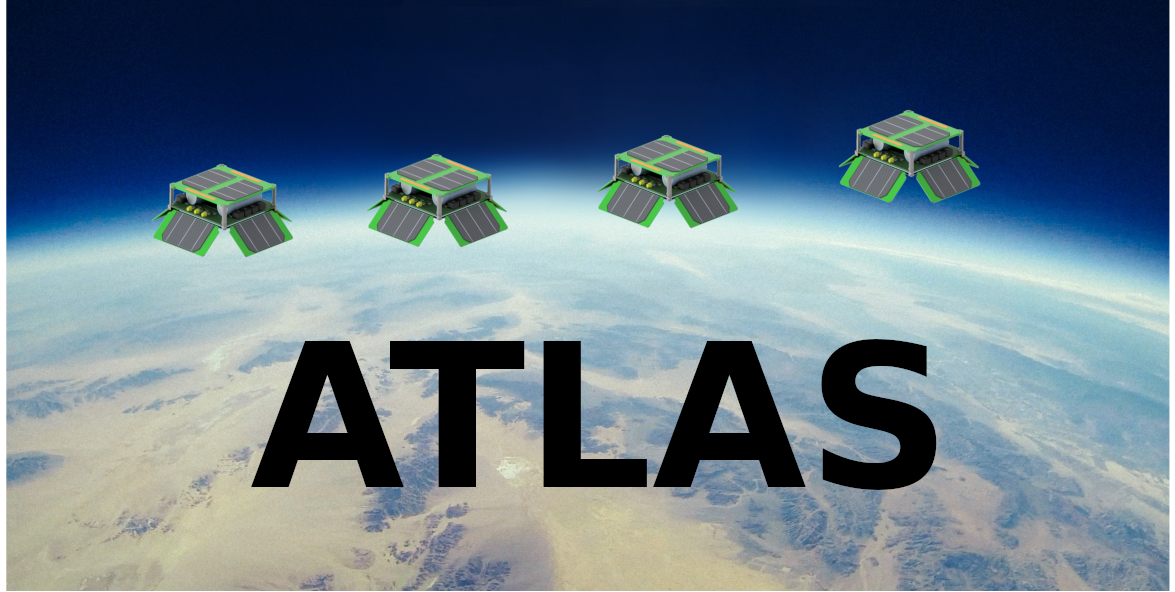
\includegraphics[width=5in]{figures/TitleImage.png} % also works with logo.pdf
    \vfill
    \vfill
\end{titlepage}

%---------------------------------------------------------------------------------
\section{Abstract}
The world around us is constantly evolving at an accelerated pace, but our understanding of our world has not been able to keep up. As technology disrupts industries, societies, and interactions, humanity's impact on the world has become so prominent we find ourselves on the verge of a 6th great extinction: The Anthropocene Era. Scientist, activists, and regulators rely on gathering global informatics in order to build accurate models, predict consequences, and plan for the future. One such system to provide this data is called ARGOS. ARGOS is a system that utilize1s low power tags on animals, glaciers, buoys, boats, etc. and a sensor package attached on polar orbiting spacecraft to determine position of those tags and to receive data. The system that is currently in place is woefully inadequate for the data needs of today and tomorrow. ATLAS is a system that is designed to augment and vastly improve the capability to locate tags, collect data, and provide continuous coverage. 

%---------------------------------------------------------------------------------
\section{Overview}

ATLAS will be a constellation of 66 autonomous 3U cube satellites that will locate and store messages from transmitting tags located anywhere around the world. The system can be subdivided into 4 sub-systems: Tags, Satellite Constellation, Gateway Terminals, and Database/Control (Figure \ref{fig:sub_flow}).
%==========================
\begin{figure}[H]
  \centering
  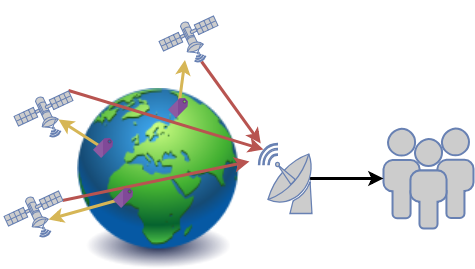
\includegraphics[width=0.8\linewidth]{figures/atlas_sub}
  \caption{ATLAS Data flow}
  \label{fig:sub_flow}
\end{figure}
%==========================
In many ways ATLAS is similar to the current Argos system, as it is fundamentally a constellation in space that collects data and location information into a database for an end user. Implementation-wise; however, ATLAS will provide a much more accurate location estimate, increased data bandwidth, and more consistent and constant global coverage. 

\subsection{Tags and Constellation}
Tags located on the ground communicate via a one-way wireless link to a satellite that is positioned along 6 orbital planes following a 350km polar orbit. Currently the ARGOS system utilizes the Doppler-shift to measure a distance from the satellite to the tag at a single instance of time. In order to determine a position at least 4 distance measurements are necessary. Collecting 4 measurements temporally spaced far enough apart can be difficult in certain situations, thus ATLAS has been designed to require only a single tag transmission to locate the object. Data bandwidth is limited in the ARGOS system because of a variety of physical constraints, the chief among them is the limited RF power output of a tag. ATLAS relaxes these constraints in three ways: lowering the altitude to reduce free-space loss, using spread-spectrum CDMA techniques to improve capacity, and utilizing different ISM allocated frequency bands to either alleviate congestion and/or reduce free-space path loss. Because ATLAS is fundamentally an orbital relay station, other techniques to increase bandwidth are possible in future system implementations. Future improvements include augmenting the system with high altitude balloons, long duration UAV flights, and/or a network of ground stations. The overall goal in an improved network compared to ARGOS is to increase the energy per bit of the transmitter either through a reduction of losses or increase in gains. 

\subsection{Gateway Terminal}
The gateway terminal side of the ATLAS system links the in-space constellation of satellites to a database from which an end-user can collect the information. These stations serve three purposes: to command and control the satellites, to down-link cached data, and to calibrate the satellites. The number of gateway stations is directly proportional  to the data bandwidth of the entire network. Initial sites for these stations include Salvabard, Norway and Northern Alaska. These two sites were chosen because far Northern (or Southern) latitudes offer a common point from which to communicate to all satellites within a single orbital period thus limiting data bandwidth limitations due to no downlink capability. Gateways can be deployed in regions that require near-real time telemetry. By placing a gateway around the region of interest the satellite constellation acts as a bent-pipe network: receiving,amplifying, and re-transmitting a tag dataset straight to the user.

\subsection{End User}
The three sub-systems described above operate as a black box from the perspective of the end-user. The constellation setup, control, timing, and networking are all handled autonomously in order to streamline the data down-link process. End users access the database via the internet which will be constantly refreshed as new data becomes available. 

\subsection{Cost}
As with any space-based system, programmatic cost is usually astronomical. These costs are exasperated when talking about a constellation because multiple satellites have a multiplicative effect on the fundamental cost of the system. Three major cost drivers in space-based missions are the hardware, launch, and operations of the satellite.
\subsubsection{Hardware}
Cubesats are much cheaper than the development and deployment of larger satellites not only because of the severe mass and volume restrictions, but also because of the potential for mass production. Unfortunately many cubesats don't realize the full cost saving potential because inherently many cubesat projects are one-off designs. The ATLAS satellite system will follow a simplistic, many-copy approach to achieve its design goals. Discussion of the hardware setup is described in the following sections. 
\subsubsection{Launch}
Although the launch cost per kilogram has been dramatically reduced due to improvements in launch vehicles, launching anything into orbit still requires a significant amount of capital. Constellations again exasperate this problem because distribution of satellites requires launches with different orbital parameters. In order to reduce the number of launches to a single launch vehicle the ATLAS satellite system will employ a propulsion system. The design chosen is further discussed in the following sections. 
\subsubsection{Operations}
For certain systems the cost to operate can become as expensive as the cost to develop and deploy. In order to minimize cost the ATLAS system will be fully automated in terms of networking, timing, down-linking data, and constellation control. This will be achieved by utilizing the gateway terminals as described previously in parallel with orbital simulations and future event predictions. 
\newpage
%---------------------------------------------------------------------------------
\section{Hardware}
ALTAS heavily employs the use of CubeSat technology by employing 3U satellites for the constellation. Each satellite is composed of 12 networked nodes that are strung together by a 20km long tether. The entire satellite can be subdivided into two subsystems: Nodes and Tether.

\subsection{3U Configuration}
A 1U cubesat configuration follows the definition that 1U is 10x10x10 cm. ATLAS utilizes a 3U configuration which is a volume constraint of 10x10x30cm and a mass constraint of 4kg. The nodes are packaged in such a way as to align pins and slots on each of the corners. When the nodes are compressed together potential energy is stored by springs. After deployment by the launch vehicle the satellite deploys one node at a time. In order to achieve passive gravity-gradient stabilization a minimum distance is required. Before stabilization is attained the tether between nodes will be slack, thus sufficient inter-node deployment velocity is required to effectively stabilize. Figure \ref{fig:node_package} shows what the 3U satellite would look like when compressed into a deployer. 

\begin{figure}[H]
  \centering
    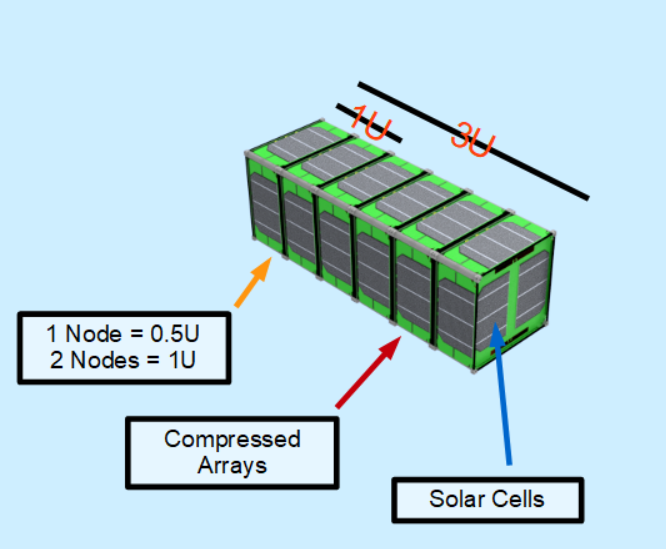
\includegraphics[width=.8\linewidth]{figures/packaged}
    \caption{Nodes packaged together. 2 nodes = 1U. Carbon fiber tether is wrapped underneath the deploy solar cells}
\label{fig:node_package}
\end{figure}

\subsection{Nodes}
Each node within the satellite are identical and can be summarized as a minimalistic, layered assembly (Figure \ref{fig:node_asm}). The nodes consist of a main body and 4 spring-deployed arrays. The main body houses a flight computer, gps, power, and communication system on two printed circuit boards sandwiching two 18650 battery cells. The 4 deployed arrays hold extra solar cells as well as patch antennas positioned off angle to increase coverage of the ground. One node is designated as the master node and communicates to the ground and dictates to the other nodes instructions as well as synchronization information.
%==========================

\begin{figure}[H]
  \centering
  \begin{subfigure}[b]{0.7\linewidth}
    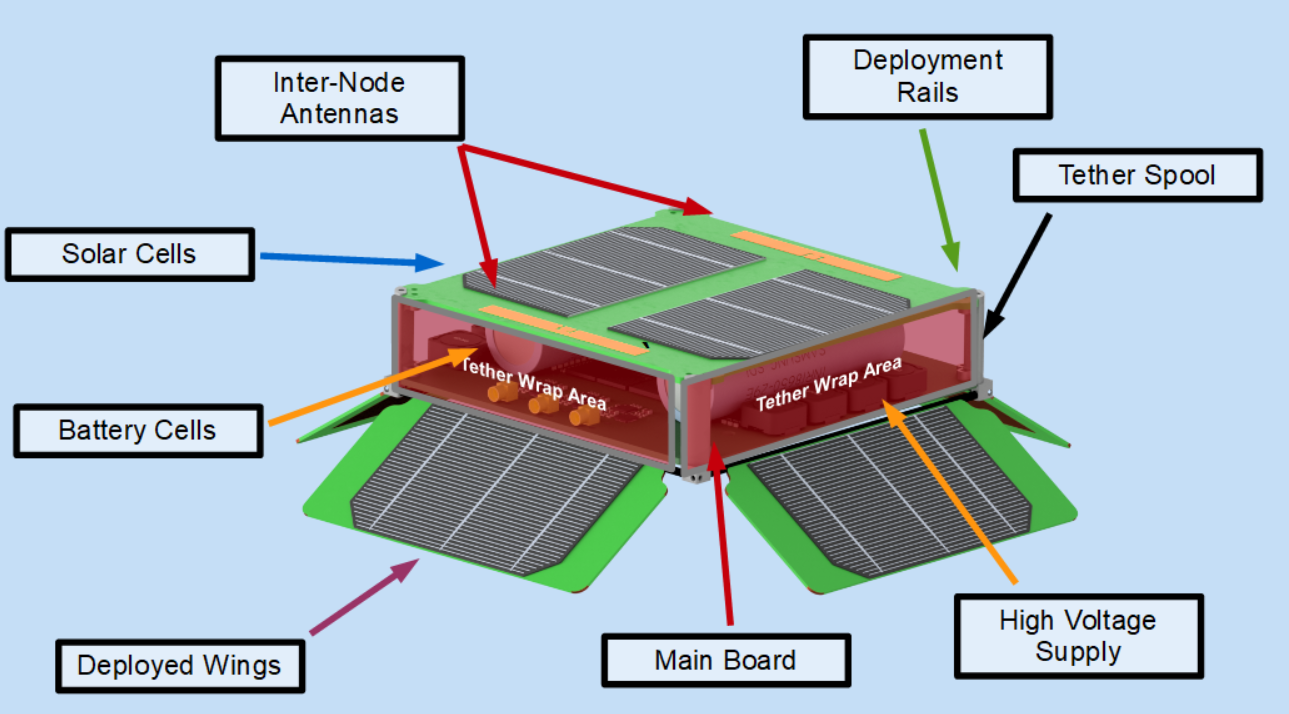
\includegraphics[width=\linewidth]{figures/Labeled_ISO}
    \caption{Major Component label}
  \end{subfigure}
  \begin{subfigure}[b]{0.7\linewidth}
    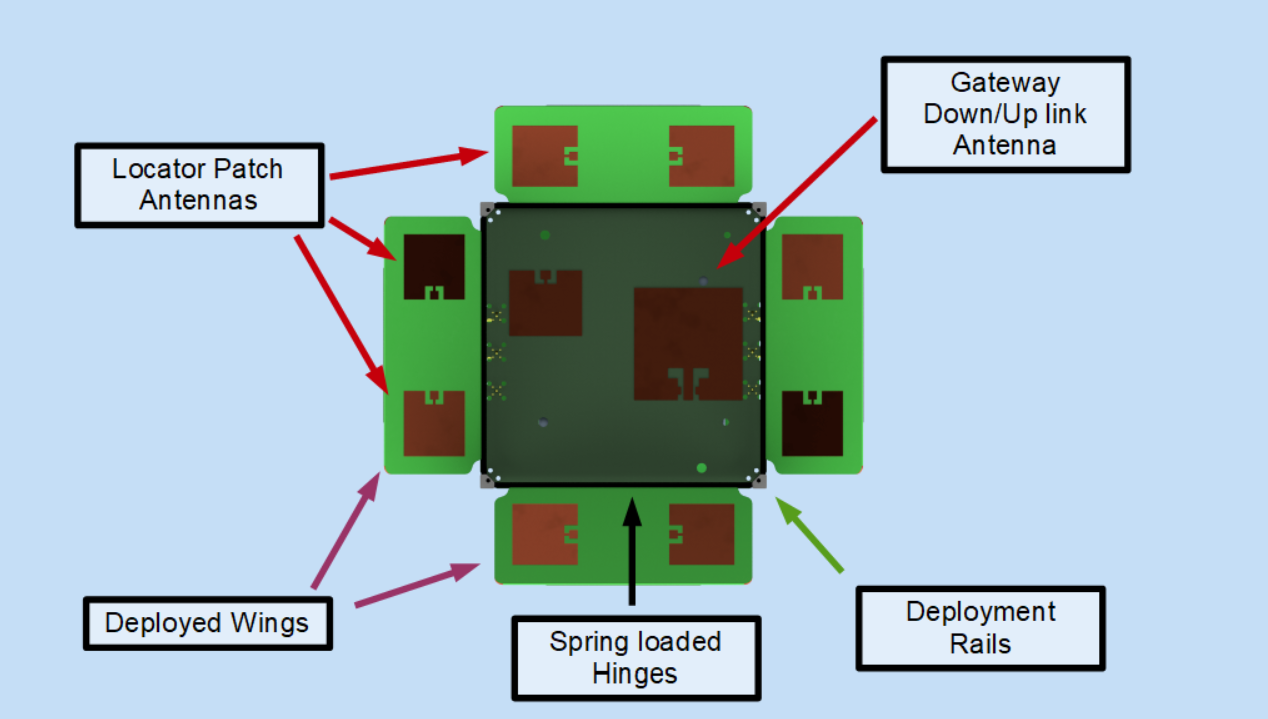
\includegraphics[width=\linewidth]{figures/Labeled_BOT}
    \caption{Bottom view}
  \end{subfigure}
  \caption{Node Overview}
  \label{fig:node_asm}
\end{figure}
%==========================
\subsection{Tether}
The tether is made out of light-weight carbon fiber thread and denotes for the largest single subsystem mass. The subsystem serves a dual purpose: to achieve passive gravity-gradient stabilization and to act as a conductive filament for an electrodynamic tether. Passive gravity-gradient stabilization utilizes the fact that gravity follows the inverse-square law which results in a tidal locking of the satellite. An electrodynamic tether is a type of thruster that utilizes the interaction between moving charges and Earth's magnetic field to impart a force onto the satellite. Through careful control of the electrodynamic tether (Figure \ref{fig:tether_moves}) it is possible to alter many orbital parameters, thus minimizing the need for multiple launches to establish the constellation. The thruster can also be used to station keep the satellite in its position as part of the constellation, and because the thruster relies on plasma in the ionosphere there are no propellant lifetime restrictions. 
%==========================
\begin{figure}[H]
  \centering
    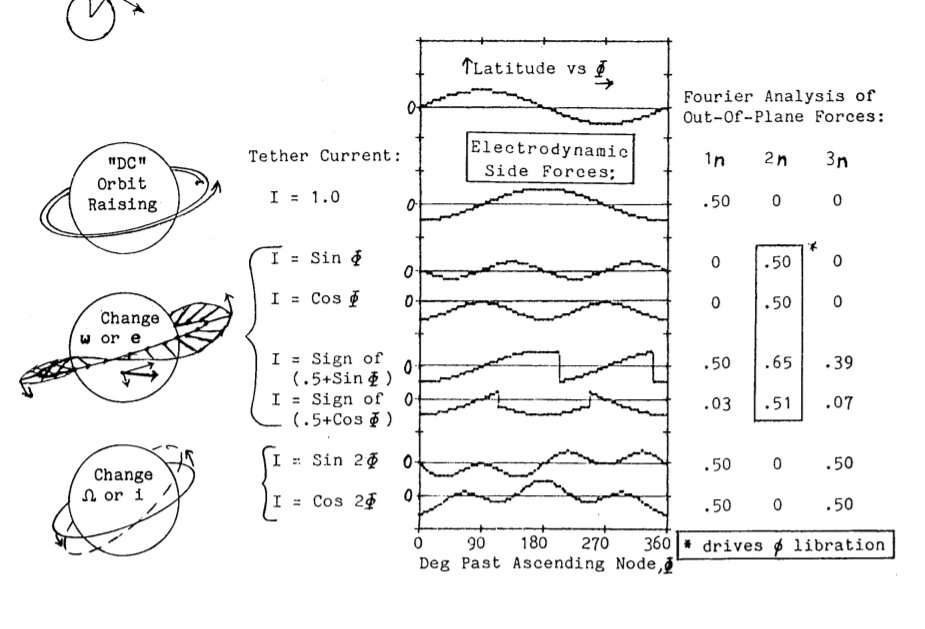
\includegraphics[width=\linewidth]{figures/tether_plane_changes}
    \caption{Thruster maneuvers (source: http://www.tethers.com/papers/TethersInSpace.pdf)}
  \label{fig:tether_moves}
\end{figure}
\begin{figure}[H]
  \centering
    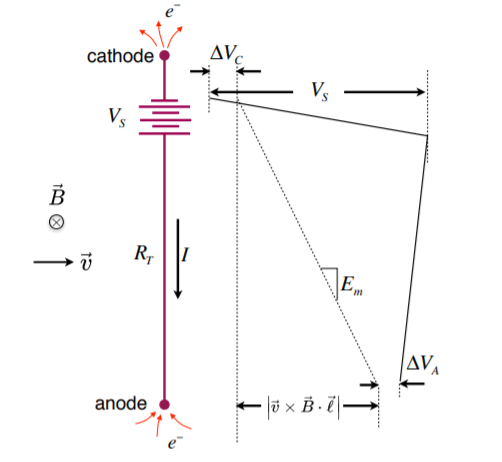
\includegraphics[width=.8\linewidth]{figures/tether_thruster}
    \caption{Thruster Physics (source: https://ocw.mit.edu/courses/aeronautics-and-astronautics/16-522-space-propulsion-spring-2015) }
\end{figure}

%==========================
\subsection{Mass Allocation}
A preliminary analysis of mass per subsystem shows which subsystem becomes the most mass intensive. Because a very long tether is required to displace the nodes the tether clearly contributes a significant factor of the mass, thus it is vital to select a material that has exceptional strength/density ratios. Fortunately with the latest aerospace push in carbon composites, readily available 1K carbon tow (unwound thread) is available weighing only 66 grams per kilometer. This can potentially be reduced as the tether strength requirements are not very stringent, possibly allowing the use of 0.5K or 0.1K tow. 
Energy storage is the next most intensive subsystem and the sizing of the energy storage device has far reaching consequences in terms of eclipse time survival, power consumption limitations, and power generation requirements. 

\begin{table}[H]
\centering
\begin{tabular}{|l|l|l|}
\hline
Item                                                        & Mass (grams)                                           & Percentage                                              \\ \hline
Tether                                                      & 1320                                                   & 33\%                                                    \\ \hline
Batteries                                                   & 1080                                                   & 27\%                                                    \\ \hline
\begin{tabular}[c]{@{}l@{}}Single Node\\ (x12)\end{tabular} & \begin{tabular}[c]{@{}l@{}}133.3\\ (1600)\end{tabular} & \begin{tabular}[c]{@{}l@{}}3.35\%\\ (40\%)\end{tabular} \\ \hline
Total                                                       & 4000                                                   & 100\%                                                   \\ \hline
\end{tabular}
\end{table}
%---------------------------------------------------------------------------------
\section{Data Path and Protocol}
The communication aspect of ATLAS is very similar to the function of cell towers utilized for the  mobile phone industry. Cell towers act as wireless gateways into a physical backbone that consists of fiber or cable, and a satellite provides a similar link between tags and gateway terminals. Figure \ref{fig:networ_sim} shows an example of a cell tower network (panel A) and the satellite constellation and the coverage of each satellite (panel B). 

%=========================
\begin{figure}[h!]
  \centering
  \begin{subfigure}[b]{0.4\linewidth}
    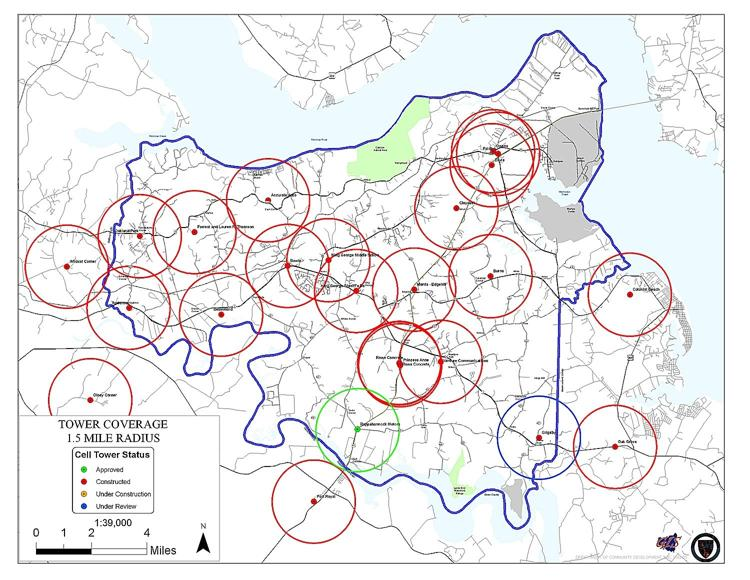
\includegraphics[width=\linewidth]{figures/cell_coverage}
    \caption{Phone/Cell Network}
  \end{subfigure}
  \begin{subfigure}[b]{0.55\linewidth}
    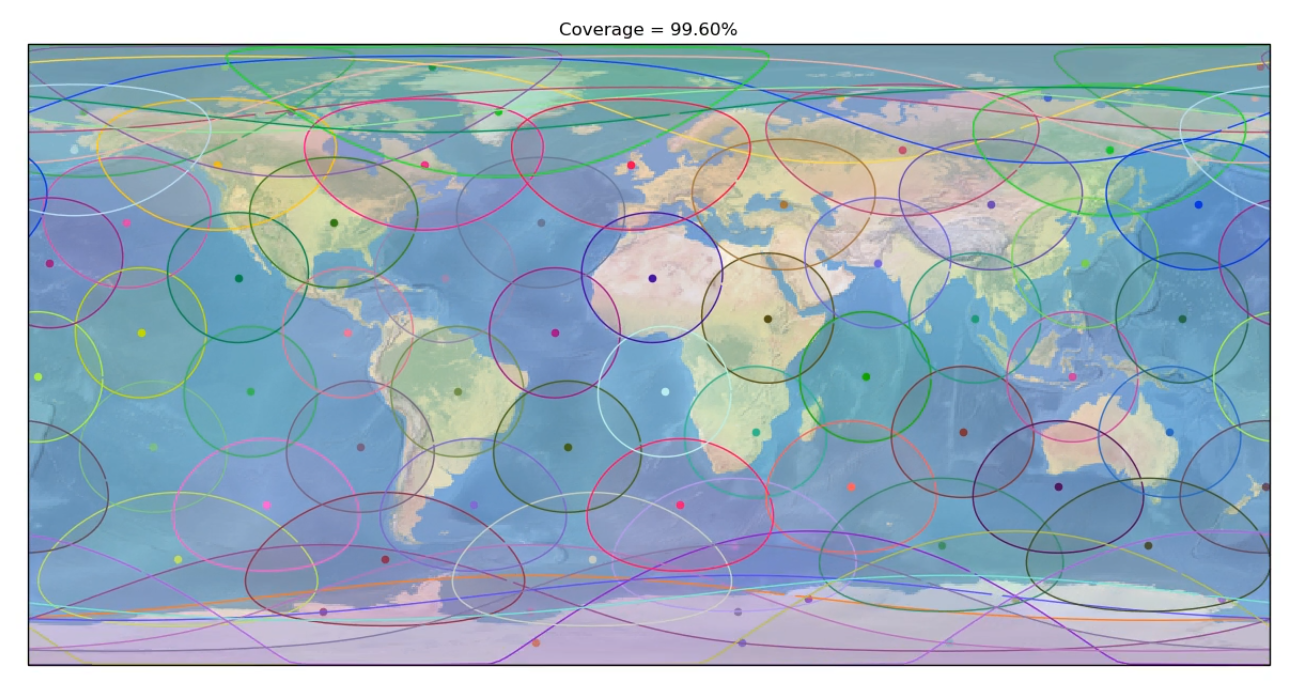
\includegraphics[width=\linewidth]{figures/350km_coverage}
    \caption{ATLAS 350km Constellation}
  \end{subfigure}
  \caption{Network Similarity}
  \label{fig:networ_sim}
\end{figure}
%===========================

Although the two networks appear similar there are several stark differences between the satellite/tag network and a phone/cell network. One such difference is that a phone/cell network is a duplex communication system (data flows both ways) while the satellite/tag network is a simplex communication system (data flows in only one direction). This means two things: the transmitters (tag) must operate without knowledge of the state of other tags and that the receiver side (satellite) and the transmitters must operate without knowledge of each other. The disadvantage of using a simplex network is that network routing/timing/state-knowledge is ambiguous; however, the advantage is a dramatic power,weight, and complexity saving on the tag side. This is what we see with transmitters utilized by the current ARGOS network with miniaturized and durable transmitters placed on the backs of the smallest of birds or the largest of whales. The ARGOS network however has severe limitations in terms of data bandwidth capability and ATLAS solves this issue in three ways: by leveraging CDMA techniques for multiple access to a single satellite, by being in a much lower orbit reducing free space path loss, and by leveraging ISM spectrum allocations for more data throughput and reduced path loss. The flow of data in the ATLAS network can be followed in the flow diagram shown in Figure \ref{fig:data_flow}.

\begin{figure}[H]
  \centering
  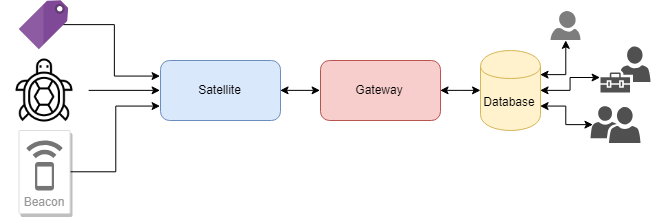
\includegraphics[width=\linewidth]{figures/data_flow}
  \caption{ATLAS Data flow}
  \label{fig:data_flow}
\end{figure}

Data is packaged and transmitted by terrestrial tags up to a satellite in low earth orbit. The satellite stores the packet on board and transmits the data when in view of a gateway terminal. The gateway terminal is connected to a server which is accessible to end-users in the form of a query database.

\subsection{Data Packet Size}
ATLAS will utilize data packets with a size of 255 bytes with a data-rate between 4800 and 9600 bits per second. 255 bytes was chosen because it is a popular data format for Reed-Solomon encoders giving room for 223 bytes for data and 32 bytes for parity. Reed-Solomon codes are codes utilized for error correction and by using a 255,223 code with 8 bit symbols it is possible to correct for up to 16 bytes of error. 

\subsection{CDMA}
When there are multiple transmitters attempting to communicate to a single receive station a method is required to make sure that the transmissions do not interfere with each other. There are three general approaches: time division multiple access (TDMA), frequency division multiple access (FDMA), and code division multiple access (CDMA). TDMA works by allocating a set time at which a transmitter sends a message. FDMA works by assigning each transmitter a portion of the frequency spectrum. CDMA involves convolving a bit stream with orthogonal  (or near orthogonal) codes so that when deconvolving is performed only one code matches. Because ATLAS is a simplex system coordinating transmission times between tags is almost impossible. Assigning frequencies to each tag is a possible solution, but would require all per-deployed tags to be recalled and properly assigned. Using CDMA allows each transmitter to receive a unique convolution code and thus the issue of multiple access is somewhat addressed. Depending on the channel bandwidth, energy per bit to noise power spectral density ratio (Eb/N0), and transmission power differences, a single CDMA channel could handle anywhere between 1 to 40 tags at a time.

\subsubsection{CDMA Power Leveling}
Cell phone systems utilize CDMA because it greatly increases the utilization of the spectrum; however, in order for CDMA to work effectively a close-loop feedback mechanism is required to maintain transmitter to receiver power levels that are nearly identical. In a simplex system this closed feed back loop is not possible. Instead we rely on two attributes: shaping the receiver antenna gain and the fact that the differences in path length in terms of dB is much less than a terrestrial system (law of small angles). The second portion results that there could be an ideal constellation geometry that minimizes differences in transmitter power levels (which increases capacity) by increasing altitude (which increases path loss).

%---------------------------------------------------------------------------------
\section{Coverage and Localization}
\subsection{Coverage}
The ATLAS constellation is a type of constellation known as “Streets-of-Coverage” which is essentially a subset configuration of a particular Walker-Delta Pattern constellation. ATLAS will provide better than 99.3\% instantaneous global coverage. The constellation consists of 6 high inclination orbital planes with 11 satellites distributed evenly across a single plane. These 11 satellites can be visualized as a ring of satellites that provide continuous coverage by overlapping their field of views (Figure \ref{fig:coverage}). 
\begin{figure}[H]
  \centering
  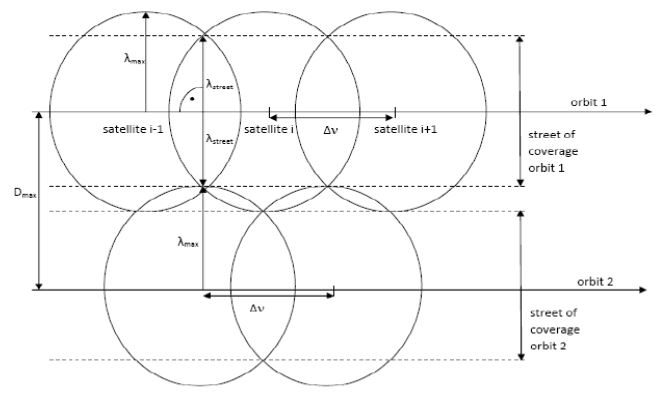
\includegraphics[width=0.65\linewidth]{figures/streets_of_coverage}
  \caption{Streets of Coverage (source: http://www.astrome.co/blogs/the-art-of-satellite-constellation-design-what-you-need-to-know/)}
\label{fig:coverage}
\end{figure}

Three configurations were considered at various altitudes: 350km, 550km and 800km. This resulted in a configuration of 6/11, 5/9, and 5/7 (\# of planes / \# of satellites per plane). As to be expected, higher altitudes result in fewer satellites; however, higher altitudes also result in higher free space path loss which results in lower data rates. Because the satellites have a method of propulsion it is possible to dynamically adjust the constellation allowing it to be resilient to satellite failures, unknown model errors, and under capacity issues. Propulsion also allows the satellites to be launched by a single launch vehicle, significantly reducing the cost of constellation setup.

The gaps in coverage provided by ATLAS are localized near the equators and when the satellites pass each other in opposite directions. The time between coverage and no-coverage is a small fraction of the pass period (less than 10 minutes). Figure \ref{fig:mask} shows the masking of what the constellation can and cannot see at a single instant of time. The black represents areas of coverage and the white represents areas outside a satellites field of view. A cost-benefit analysis could be done to argue that a configuration of 7/12 could resolve this issue; however, any over-optimization results in a more expensive system. 

\begin{figure}[H]
  \centering
    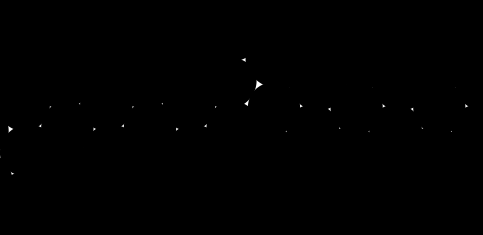
\includegraphics[width=0.5\linewidth]{figures/masking}
    \caption{Gaps in coverage at a single time instant}
  \label{fig:mask}
\end{figure}

The video link provided shows these altitude runs over a single orbital period.
\begin{figure}[H]
  \centering
  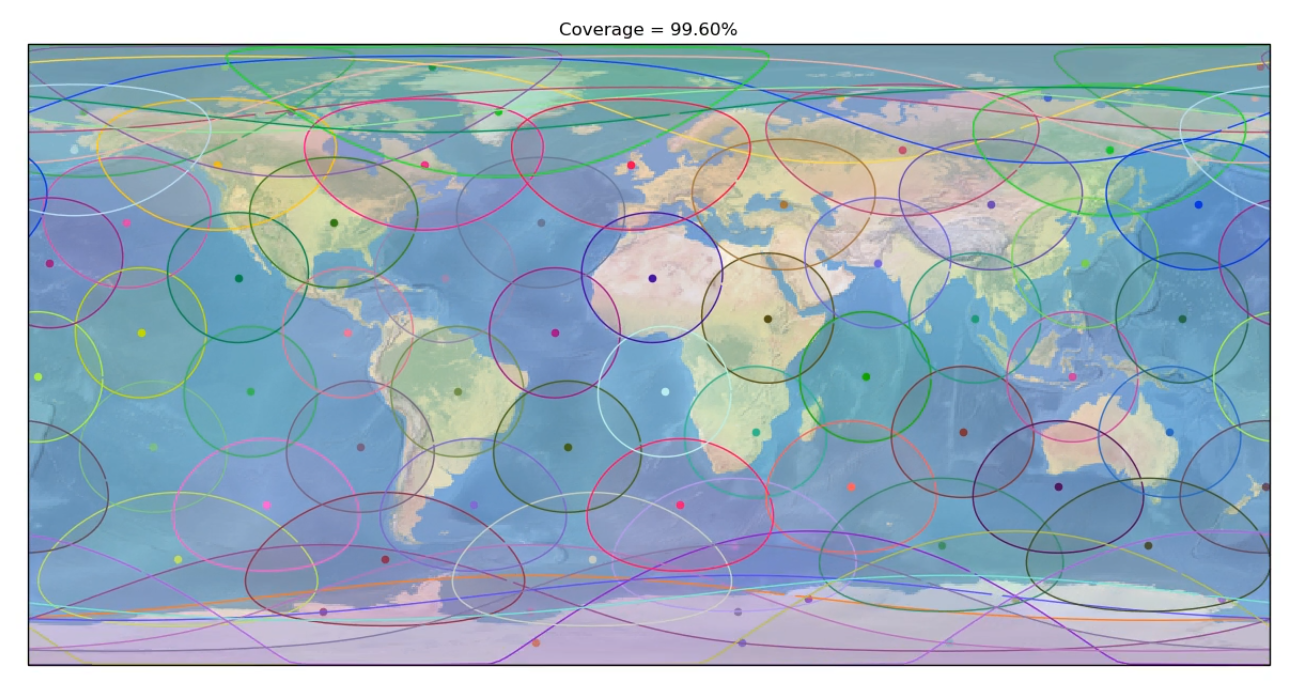
\includegraphics[width=\linewidth]{figures/350km_coverage}
  \caption{350km Altitude | 66 Satellites | 6/11}
\end{figure}
\begin{figure}[H]
  \centering
  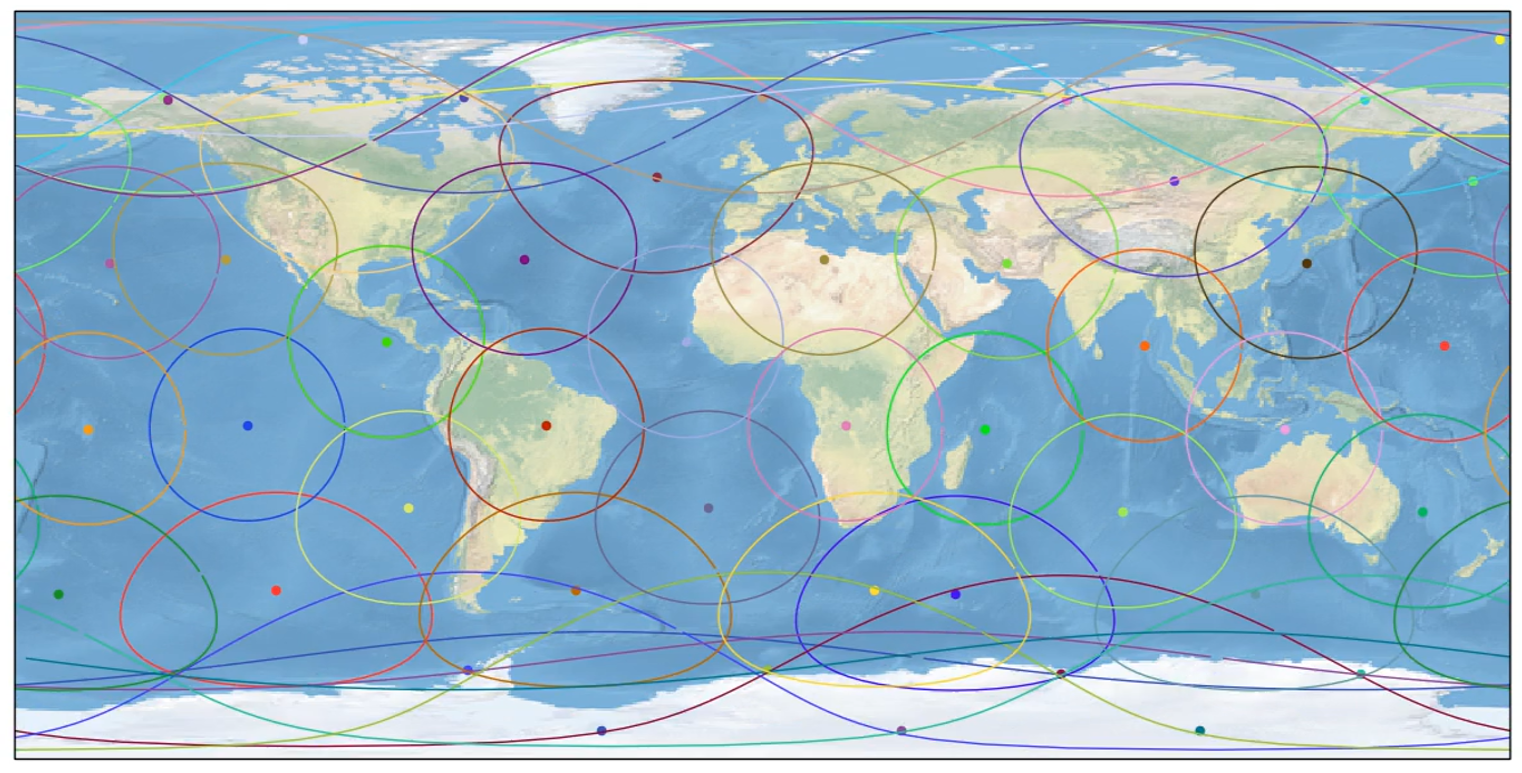
\includegraphics[width=\linewidth]{figures/500km_coverage}
  \caption{550km Altitude | 45 Satellites | 5/9}
\end{figure}
\begin{figure}[H]
  \centering
  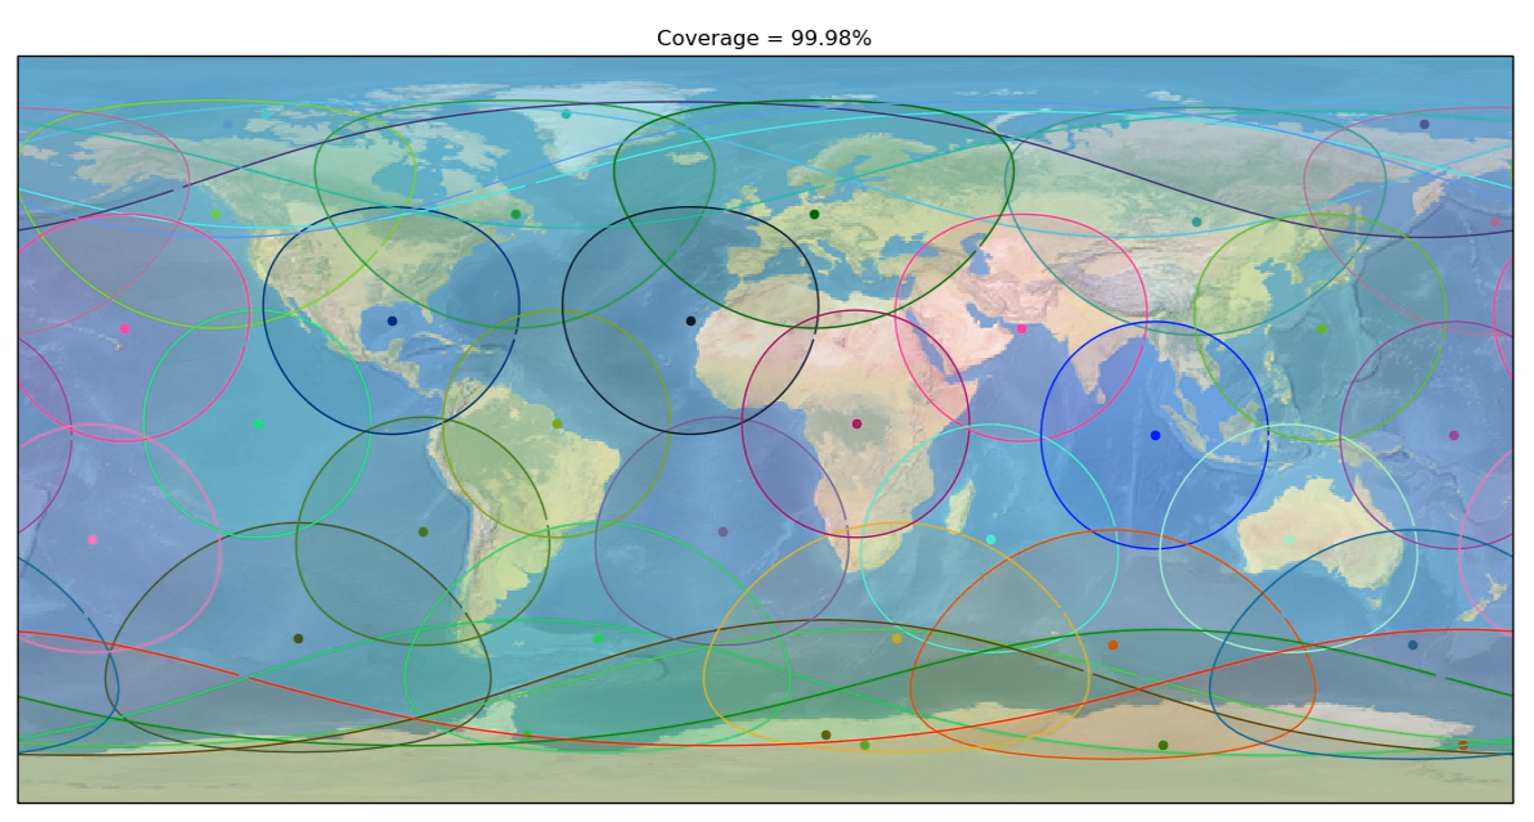
\includegraphics[width=\linewidth]{figures/800km_coverage}
  \caption{800km Altitude | 35 Satellites | 5/7}
\end{figure}

\subsection{Localization}
A single satellite within the ATLAS constellation can provide the location of a tag given a single message using Time Difference of Arrival (TDOA) localization. The spatial accuracy of the ATLAS constellation is modeled to be on average +/- 74 meters. 

TDOA can determine the position of a transmitting source through knowledge of the wave velocity (speed of light) and the positions of at least 4 receiving stations as shown in Figure \ref{fig:tdoa}. Multiple variables influence the accuracy of such a system with the two largest influences being the receivers' relative position (geometry of the satellite) and timing synchronization between receivers. 

\begin{figure}[H]
  \centering
  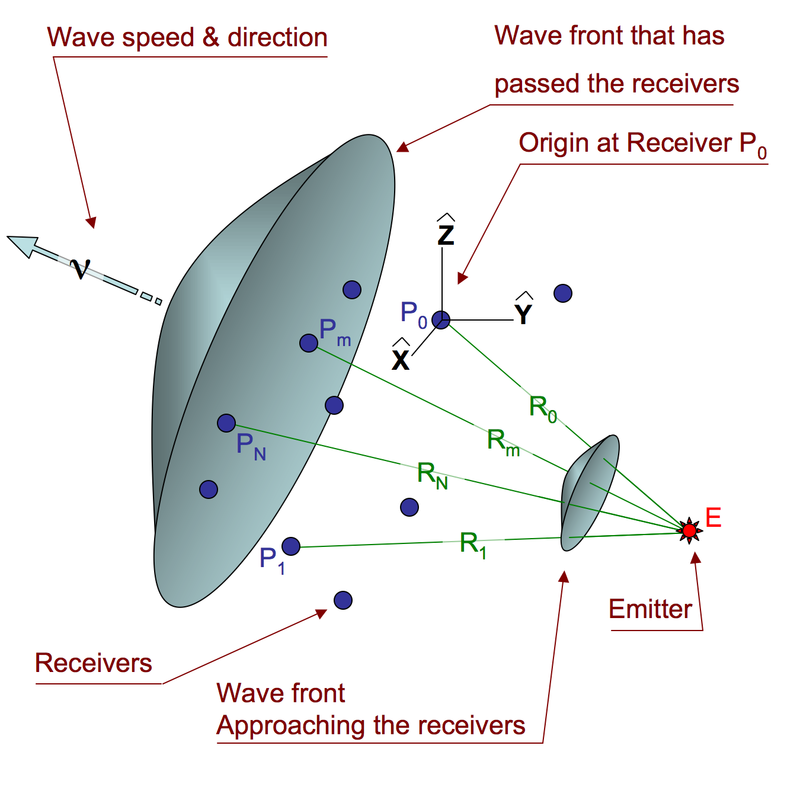
\includegraphics[width=0.65\linewidth]{figures/TDOA_Geometry}
  \caption{TDOA wavefront timing example (source: https://en.wikipedia.org/wiki/Multilateration)}
\label{fig:tdoa}
\end{figure}

As explained earlier, a single satellite consists of 12 nodes along a 20km tether. The on-orbit position of these nodes with respect to each other is affected by the distribution of nodes along the tether, drag forces experienced by each node, stretching and thermal affects on the tether, as well as a variety of other diminishing factors. By pseudo-randomly distributing the nodes along the tether it is possible to achieve an almost random distribution of nodes within a constrained space. This is important because in order to solve the system of non-linear equations accurately it is best if the positions between nodes is as independent as possible.

Timing synchronization between nodes is done via an inter-node wireless network and is one of the more challenging technical problem to be solved. Terrestrial wireless networks are capable of +/- 50ps synchronization. With a timing accuracy of +/- 100ps we can achieve +/- 75 meter accuracy. With an accuracy of 1ns it is possible to achieve +/- 800 meter accuracy. There are a variety of methods to achieve sub-nanosecond timing. One option is a master node transmits a reference CW radio wave that each node then subsequently latches onto using a phase-locked loop. A second network is utilized to communicate data between nodes until down-link by the master node to the gateway terminal. 

\subsubsection{Model Results}
The following figures show some simulation results given various altitude, node quantity, and timing noise characterization. Timing noise was modeled as a gaussian distribution given a standard deviation value centered around 0. The overdetermined system of non-linear equations is solved iteratively using a trust region reflective algorithm.

\begin{figure}[H]
  \centering
  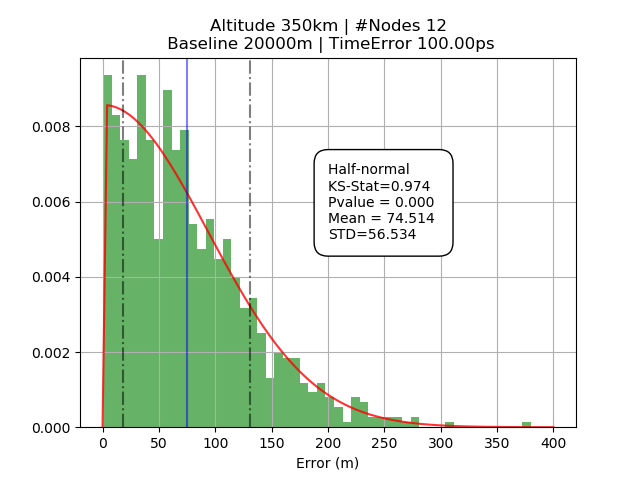
\includegraphics[width=.75\linewidth]{figures/graphs/350_12_20000_100}
  \caption{Selected Constellation Design}
\end{figure}

%%%%%%%%%%%%%%%%%%%%%%
\subsubsection{Effect of Node Quantity}
\begin{figure}[H]
  \centering
  \begin{subfigure}[b]{0.49\linewidth}
    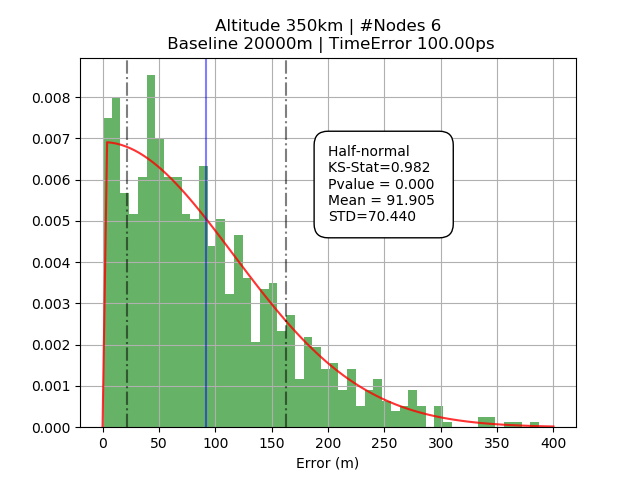
\includegraphics[width=\linewidth]{figures/graphs/350_6_20000_100}
  \end{subfigure}
  \begin{subfigure}[b]{0.49\linewidth}
    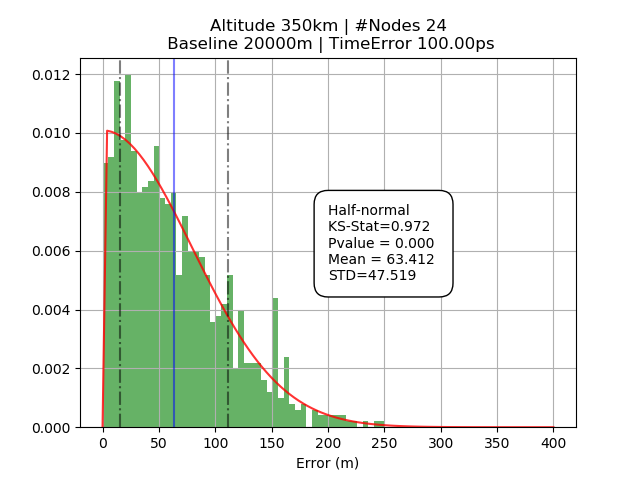
\includegraphics[width=\linewidth]{figures/graphs/350_24_20000_100}
  \end{subfigure}
\end{figure}

%%%%%%%%%%%%%%%%%%%%%%
\subsubsection{Effect of Altitude}
\begin{figure}[H]
  \centering
  \begin{subfigure}[b]{0.49\linewidth}
    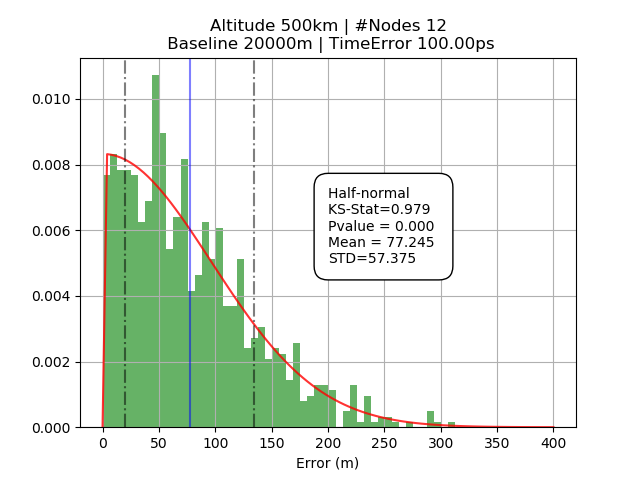
\includegraphics[width=\linewidth]{figures/graphs/500_12_20000_100}
  \end{subfigure}
  \begin{subfigure}[b]{0.49\linewidth}
    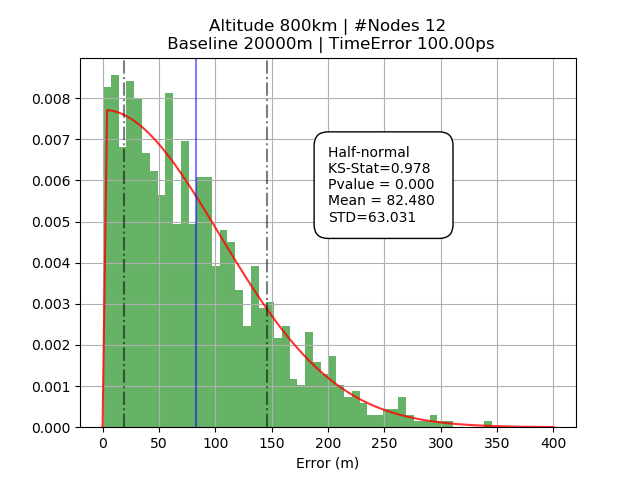
\includegraphics[width=\linewidth]{figures/graphs/800_12_20000_100}
  \end{subfigure}
\end{figure}

%%%%%%%%%%%%%%%%%%%%%%
\subsubsection{Effect of Tether Length}
\begin{figure}[H]
  \centering
  \begin{subfigure}[b]{0.49\linewidth}
    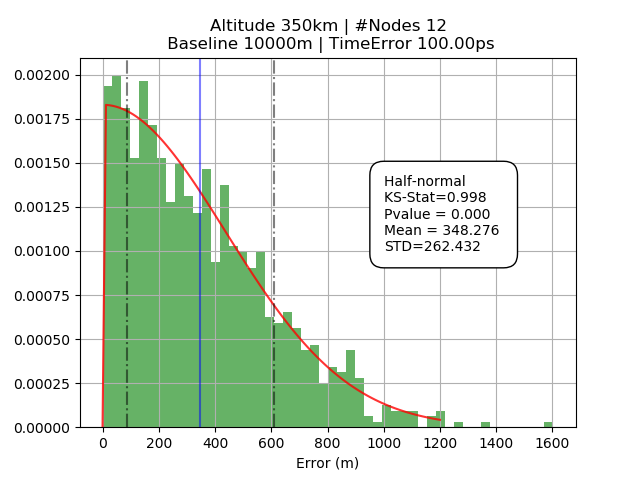
\includegraphics[width=\linewidth]{figures/graphs/350_12_10000_100}
  \end{subfigure}
  \begin{subfigure}[b]{0.49\linewidth}
    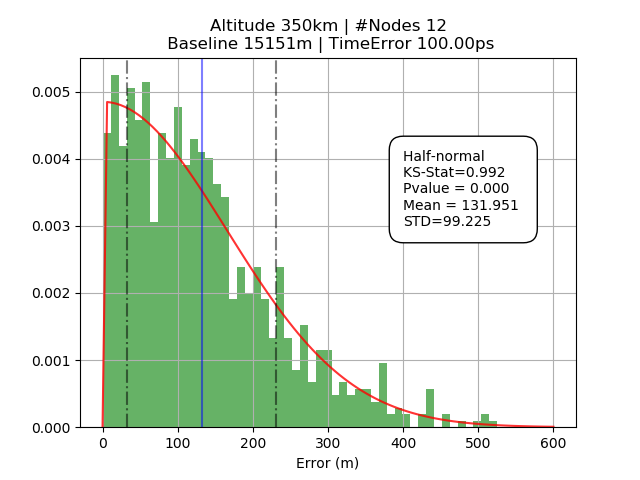
\includegraphics[width=\linewidth]{figures/graphs/350_12_15151_100}
  \end{subfigure}
\end{figure}

%%%%%%%%%%%%%%%%%%%%%%
\subsubsection{Effect of Timing Error}
\begin{figure}[H]
  \centering
  \begin{subfigure}[b]{0.49\linewidth}
    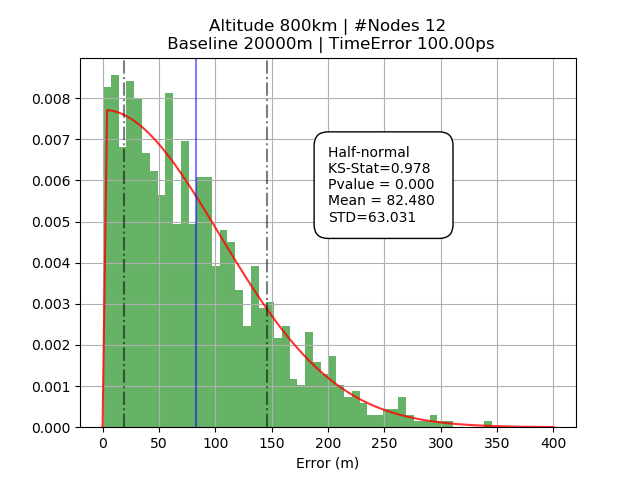
\includegraphics[width=\linewidth]{figures/graphs/800_12_20000_100}
  \end{subfigure}
  \begin{subfigure}[b]{0.49\linewidth}
    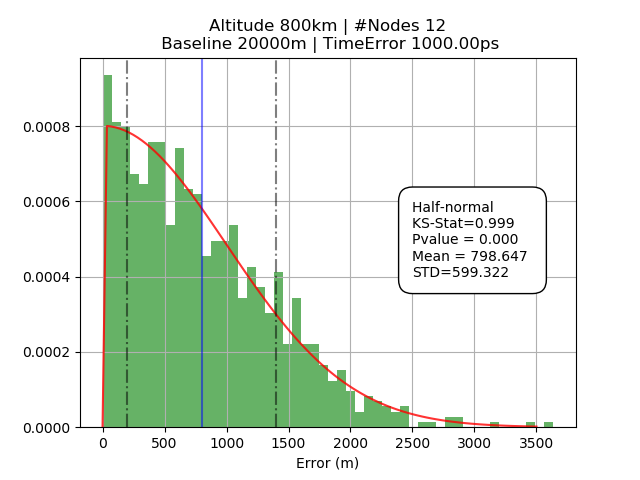
\includegraphics[width=\linewidth]{figures/graphs/800_12_20000_1000}
  \end{subfigure}
\end{figure}
%---------------------------------------------------------------------------------
\section{Open Source Standard}
The ATLAS system is designed with an open source attitude in mind with no proprietary hardware or software constraints. In order to fully utilize a global system it is best if all users involved can fully integrate and iterate new and better designs quickly. That being said it is prudent that transmitters are properly vetted and validated before being deployed to ensure that one faulty transmitter doesn't cause area-wide lock out. 

\section{Future Work}
As a preliminary survey of an ambitious idea, the feasibility of a constellation formed by a series of tethered satellite nodes seems plausible. Currently under development is a refinement of the orbital simulation model to include a link budget calculation in order to develop a data throughput model. Other in progress updates include improving the least-squares localization algorithm to be more robust to incorrect boundary conditions. Although tethered satellites have been designed and deployed there is very little technical research into electrodynamic tethers. More research is warranted to investigate this mode of propulsion, which could greatly expand the capabilities of any cubesatellite system. 

\end{document}
